\begin{figure}
  \centering
  \captionsetup{justification=centering}
  \begin{subfigure}[t]{0.75\linewidth}
    \label{subfig:top_view}
    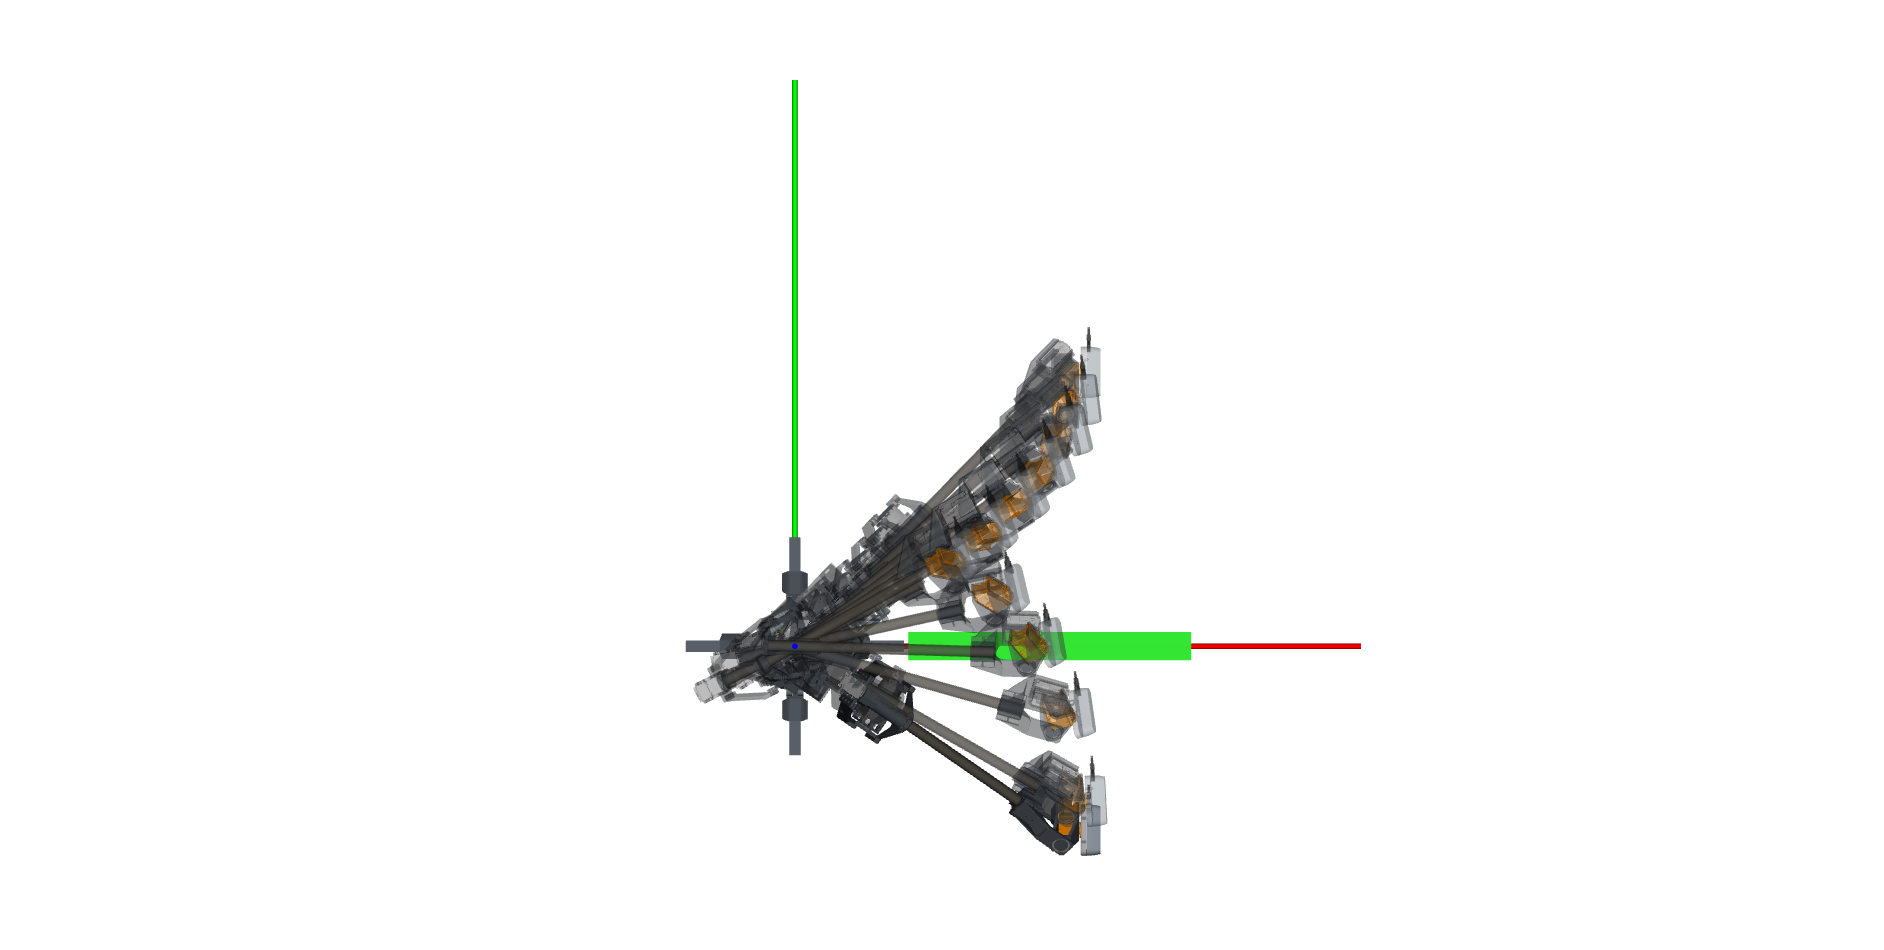
\includegraphics[width=\linewidth]{benchmark_simulation_top.png}
     \caption{}
  \end{subfigure}
  \begin{subfigure}[t]{0.75\linewidth}
    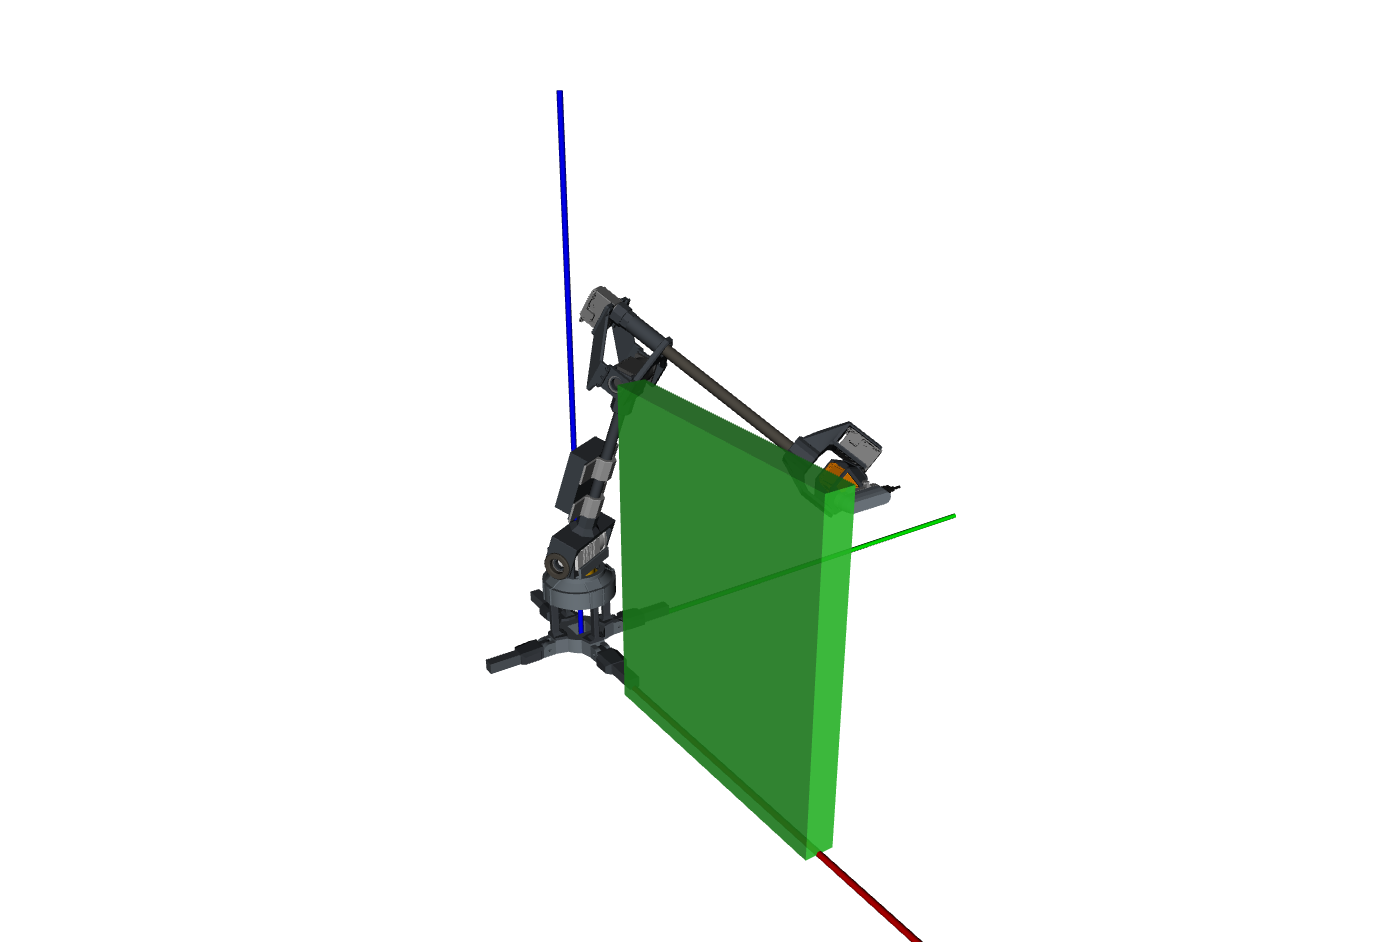
\includegraphics[width=\linewidth]{benchmark_simulation_iso2.png}
    \caption{}
  \end{subfigure}
  \begin{subfigure}[t]{0.75\linewidth}
    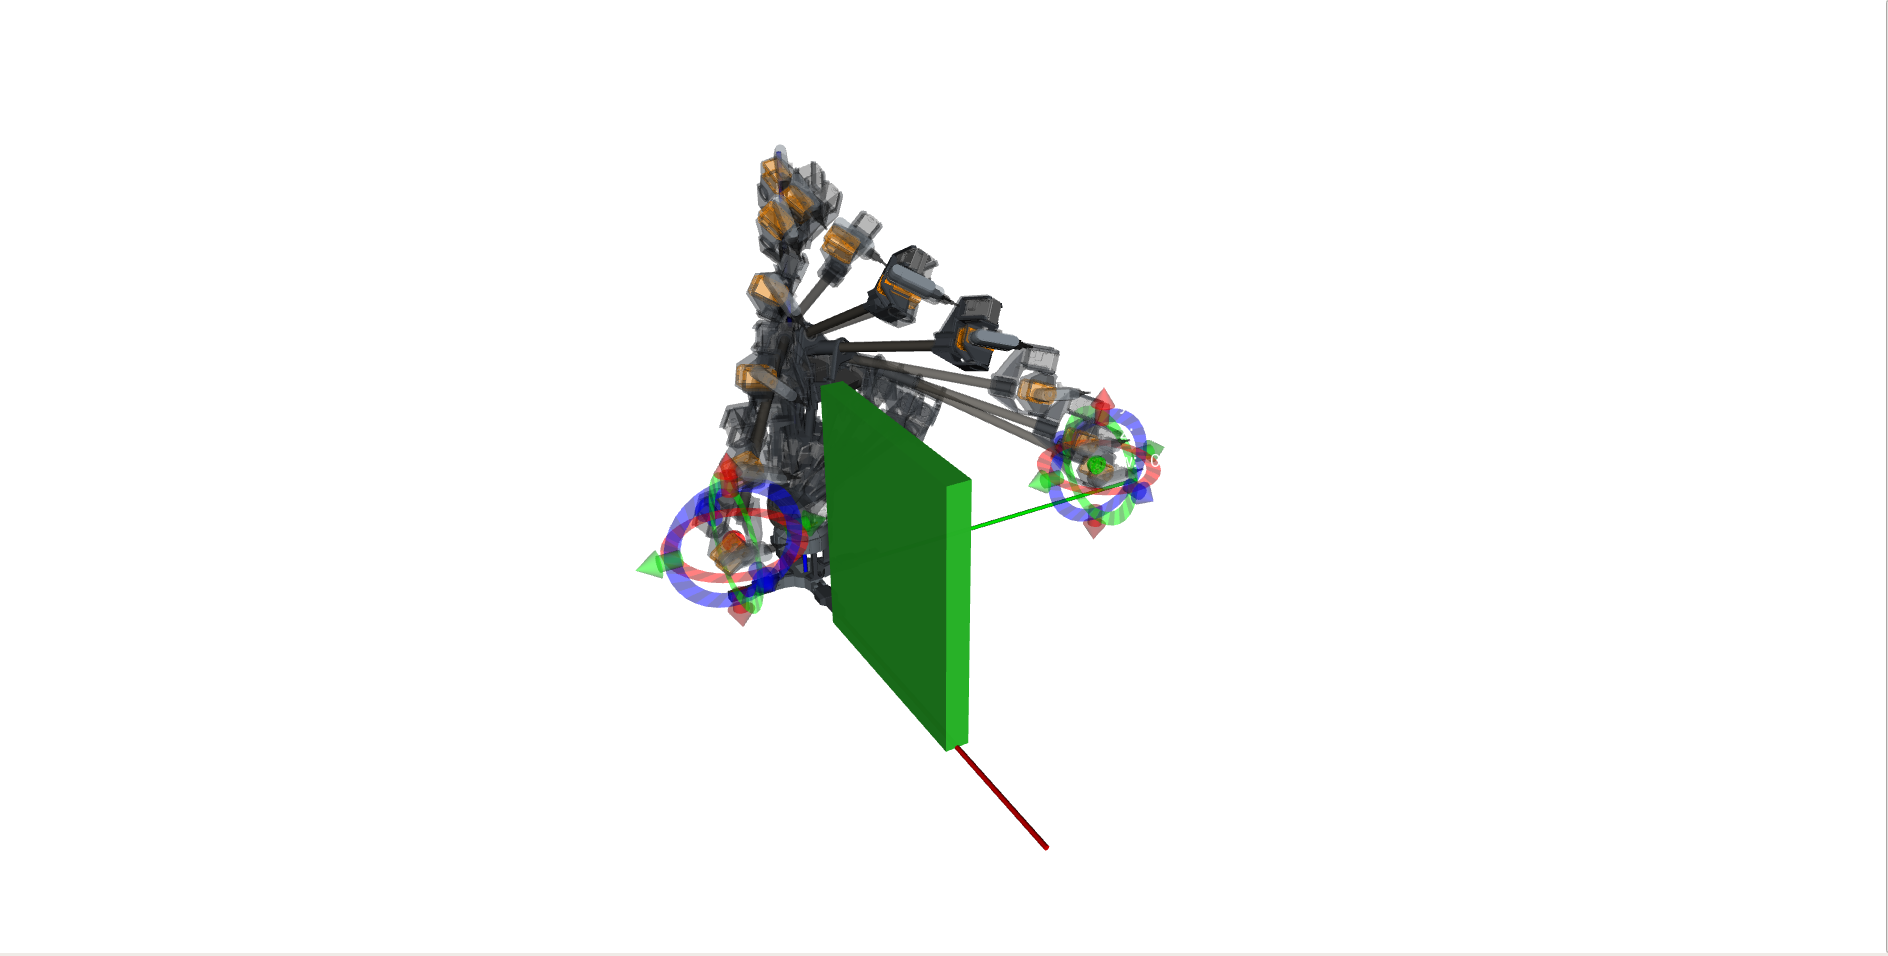
\includegraphics[width=\linewidth]{benchmark_avoiding_obs.png}
    \caption{}
  \end{subfigure}
  \caption{The top view of the simulation shown in ,(a) , 
  and the isometric view of the benchmark setup in (b).
  In (c) \rimini \ attempts to move
     around the static obstacle placed in it's immediate configuration workspace.}
  \label{fig:benchmark_simulation}
\end{figure}
